\documentclass[tikz,border=10pt]{standalone}
% Shared preamble for the CenterTask panel files (panel_a/b/c.tex).
% Edit colours and node styles here, once.
\usepackage{amsmath}
\usetikzlibrary{arrows.meta,positioning,calc}

% category colours as in ColorCategoryMap.m: 1=Short/Orange, 2=Mid/Green, 3=Long/Blue
\definecolor{catShort}{RGB}{243,178,132}
\definecolor{catMid}{RGB}{158,209,172}
\definecolor{catLong}{RGB}{157,188,234}

\tikzset{ctpanel/.style={
  font=\sffamily,
  band/.style={rounded corners=6pt, fill=black!7, draw=none, inner sep=8pt, minimum height=1.15cm},
  unit/.style={circle, fill=catMid!60, draw=none, minimum size=0.95cm, inner sep=0pt},
  flow/.style={-{Latex[length=2.2mm]}, line width=0.8pt},
  rowlab/.style={anchor=east, font=\sffamily\large},
  now/.style={fill=catShort!55, rounded corners=3pt, inner sep=3pt},
  stage/.style={rounded corners=6pt, fill=black!8, draw=none, inner sep=8pt, minimum height=1.2cm, align=center},
  target/.style={circle, minimum size=0.9cm, inner sep=0pt, draw=none, font=\sffamily\scriptsize, text=black!75},
  axis/.style={line width=0.6pt},
}}


% ---------------------------------------------------------------------
%  Our two networks drawn in the textbook "many-to-many, T_x = T_y"
%  layout (green x^{<t>}, blue a^{<t>}, red y^{<t>}, a^{<0>} on the left).
%  a^{<t>} is the hidden state (our h_t / g(t)); y^{<t>} the output.
% ---------------------------------------------------------------------

\definecolor{ngGreen}{RGB}{217,234,211}
\definecolor{ngGreenLine}{RGB}{106,168,79}
\definecolor{ngBlue}{RGB}{207,226,243}
\definecolor{ngBlueLine}{RGB}{111,168,220}
\definecolor{ngRed}{RGB}{244,204,204}
\definecolor{ngRedLine}{RGB}{224,102,102}

\begin{document}
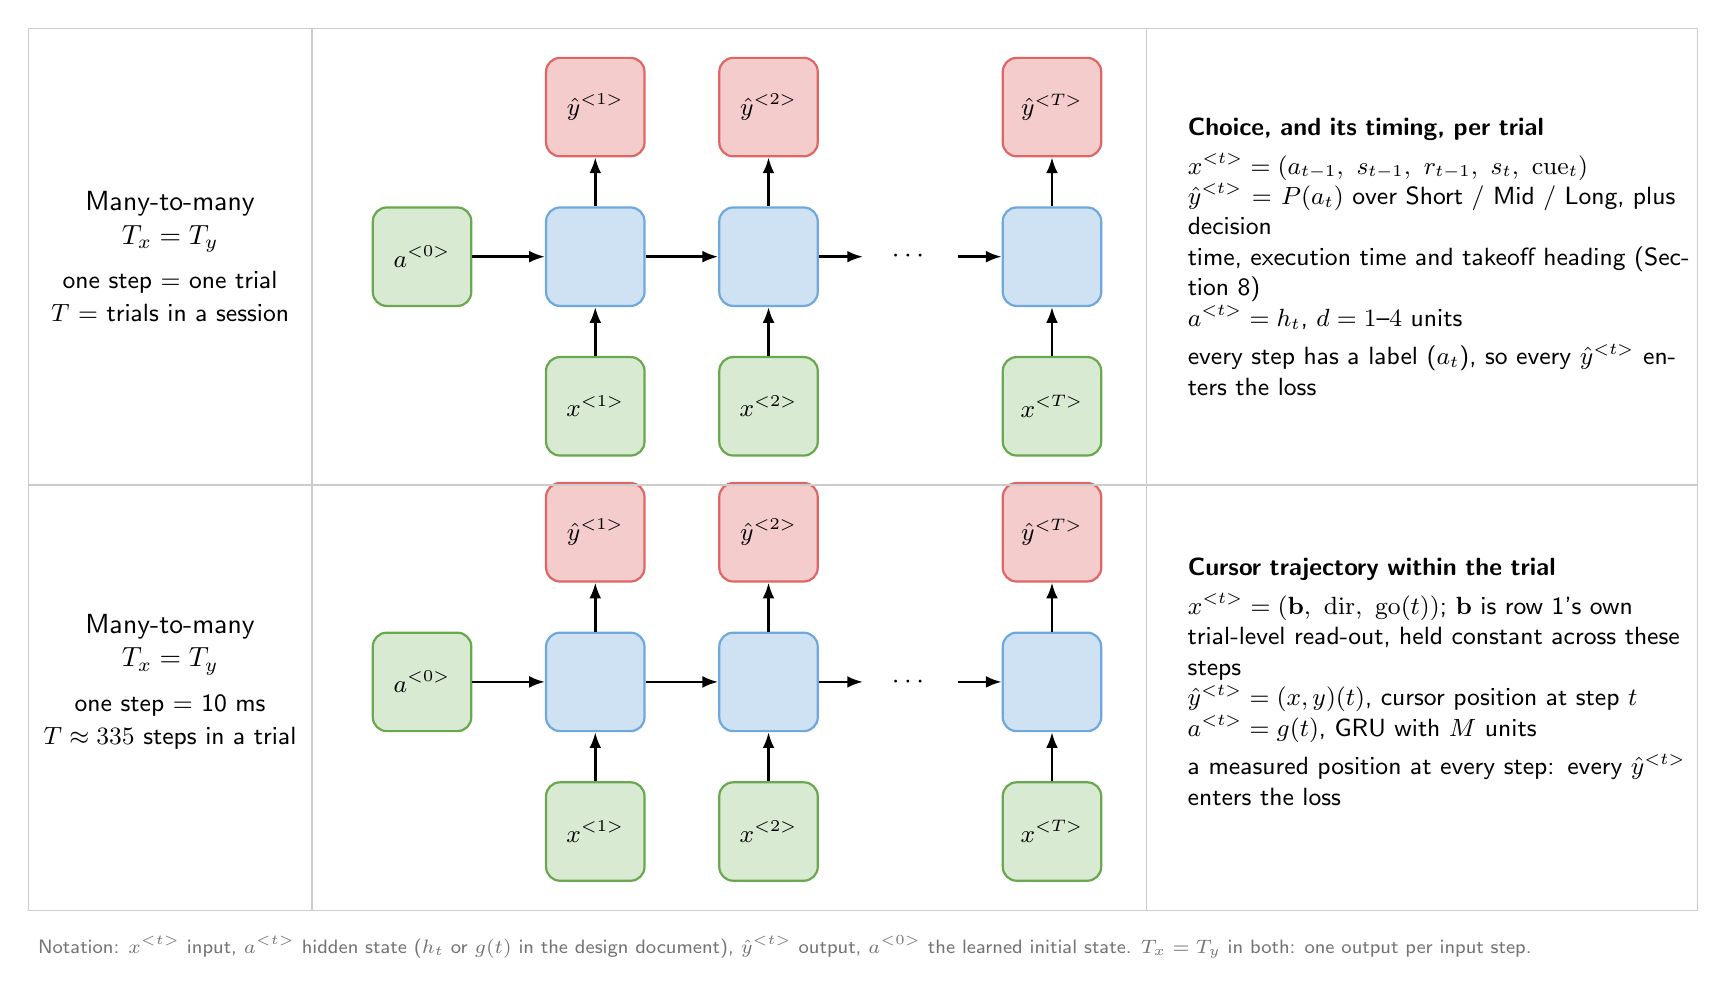
\begin{tikzpicture}[
  font=\sffamily,
  xbox/.style={rounded corners=5pt, draw=ngGreenLine, line width=0.8pt, fill=ngGreen, minimum width=1.25cm, minimum height=1.25cm, font=\small},
  abox/.style={rounded corners=5pt, draw=ngBlueLine,  line width=0.8pt, fill=ngBlue,  minimum width=1.25cm, minimum height=1.25cm},
  ybox/.style={rounded corners=5pt, draw=ngRedLine,   line width=0.8pt, fill=ngRed,   minimum width=1.25cm, minimum height=1.25cm, font=\small},
  arr/.style={-{Latex[length=2mm]}, line width=0.9pt},
  left/.style={font=\sffamily, align=center, anchor=center},
  right/.style={font=\sffamily\small, align=left, anchor=west, text width=6.4cm},
  grid/.style={black!20, line width=0.5pt},
]

% one unrolled column: #1 id, #2 x coord, #3 x label, #4 y label, #5 y style
\newcommand{\col}[5]{%
  \node[xbox] (x#1) at (#2, 0)   {#3};
  \node[abox] (a#1) at (#2, 1.9) {};
  \node[#5]   (y#1) at (#2, 3.8) {#4};
  \draw[arr] (x#1) -- (a#1);
  \draw[arr] (a#1) -- (y#1);
}

% ======================= row 1: trial-level tiny RNN =======================
\begin{scope}[yshift=5.4cm]
  \node[left] at (-3.2,1.9) {Many-to-many\\ $T_x = T_y$\\[4pt] {\small one step = one trial}\\ {\small $T$ = trials in a session}};
  \node[xbox] (a0) at (0,1.9) {$a^{<0>}$};
  \col{1}{2.2}{$x^{<1>}$}{$\hat y^{<1>}$}{ybox}
  \col{2}{4.4}{$x^{<2>}$}{$\hat y^{<2>}$}{ybox}
  \node at (6.2,1.9) {$\cdots$};
  \col{3}{8.0}{$x^{<T>}$}{$\hat y^{<T>}$}{ybox}
  \draw[arr] (a0) -- (a1);
  \draw[arr] (a1) -- (a2);
  \draw[arr] (a2) -- (5.6,1.9);
  \draw[arr] (6.8,1.9) -- (a3);
  \node[right] at (9.6,1.9) {\textbf{Choice, and its timing, per trial}\\[3pt]
    $x^{<t>} = (a_{t-1},\ s_{t-1},\ r_{t-1},\ s_t,\ \mathrm{cue}_t)$\\
    $\hat y^{<t>} = P(a_t)$ over Short / Mid / Long, plus decision\\ time, execution time and takeoff heading (Section 8)\\
    $a^{<t>} = h_t$, $d = 1$--$4$ units\\[3pt]
    every step has a label ($a_t$), so every $\hat y^{<t>}$ enters the loss};
\end{scope}

% ======================= row 2: motor (joystick) network =======================
\begin{scope}[yshift=0cm]
  \node[left] at (-3.2,1.9) {Many-to-many\\ $T_x = T_y$\\[4pt] {\small one step = 10 ms}\\ {\small $T \approx 335$ steps in a trial}};
  \node[xbox] (c0) at (0,1.9) {$a^{<0>}$};
  \col{1}{2.2}{$x^{<1>}$}{$\hat y^{<1>}$}{ybox}
  \col{2}{4.4}{$x^{<2>}$}{$\hat y^{<2>}$}{ybox}
  \node at (6.2,1.9) {$\cdots$};
  \col{3}{8.0}{$x^{<T>}$}{$\hat y^{<T>}$}{ybox}
  \draw[arr] (c0) -- (a1);
  \draw[arr] (a1) -- (a2);
  \draw[arr] (a2) -- (5.6,1.9);
  \draw[arr] (6.8,1.9) -- (a3);
  \node[right] at (9.6,1.9) {\textbf{Cursor trajectory within the trial}\\[3pt]
    $x^{<t>} = (\mathbf{b},\ \mathrm{dir},\ \mathrm{go}(t))$; $\mathbf{b}$ is row 1's own\\ trial-level read-out, held constant across these steps\\
    $\hat y^{<t>} = (x, y)(t)$, cursor position at step $t$\\
    $a^{<t>} = g(t)$, GRU with $M$ units\\[3pt]
    a measured position at every step: every $\hat y^{<t>}$ enters the loss};
\end{scope}

% ======================= table grid, as in the textbook figure =======================
\draw[grid] (-5.0,-1.0) rectangle (16.2,10.2);
\draw[grid] (-5.0,4.4) -- (16.2,4.4);
\draw[grid] (-1.4,-1.0) -- (-1.4,10.2);
\draw[grid] (9.2,-1.0) -- (9.2,10.2);

\node[font=\sffamily\scriptsize, text=black!55, anchor=north west] at (-5.0,-1.2)
  {Notation: $x^{<t>}$ input, $a^{<t>}$ hidden state ($h_t$ or $g(t)$ in the design document), $\hat y^{<t>}$ output, $a^{<0>}$ the learned initial state. $T_x = T_y$ in both: one output per input step.};

\end{tikzpicture}
\end{document}
